\section{XILINX VIVADO Report}
In this chapter will be presented the results obtained by creating a project with \textbf{Xilin VIVADO} by selecting the Zybo Zynq-7000 (xc7z010clg400-1) as working device. As will be highlighted by the resource utilization paragraph, the \textbf{Implementation phase has not been performed} due to the fact that the \textbf{Zybo-Board} does not have enough inputs and outputs ports: in our case we need 10*8 + 11*9 = 179 input pins (even if we fix the weights there is a need of 99 input pins) with only 4 slides switches and 4 push-buttons available to drive the inputs. All things considered the results that will be shown in this chapter are obtained after the \textbf{Synthesis phase} with the timing (clock) constraint.

\subsection{RTL Analysis}
Before heading with the Synthesis a preliminary double-check of the correctness of the system has been made by simply comparing the schemas obtained by the \textbf{Elaborated Design} with the ones in shown in the architecture chapter.\textbf{ No problems has been found at this stage} (in the project folder can be seen all the schemas in pdf format).
\subsection{Timing Report}
After running the Synthesis command after adding the clock constraint the following Timing Report has been displayed:
\begin{figure}[H]
	\centering
	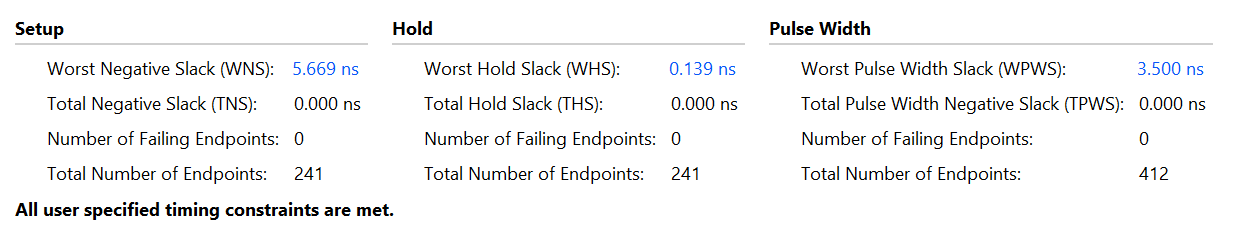
\includegraphics[width=\textwidth]{img/vivado/timing.png}
	\caption{Timing Report}
\end{figure}
As we can see the Worst Negative Slack (WNS) is \textbf{positive}, so we can drive the board at an higher frequency than 125MHz. We can calculate the \textbf{maximum frequency} as:
\begin{equation}
	f_{max} = \frac{1}{T_{clk} - WNS} = 429.0 MHz
\end{equation}
$T_{clk}$ is given by the Zybo Board which operates with 125 MHz and, for this reason, will grant an $T_{clk} = 1/125MHz = 8ns$. The WSN is determined by the \textbf{Critical Path} of the architecture which is shown in the following table (see first row):
\begin{figure}[H]
	\centering
	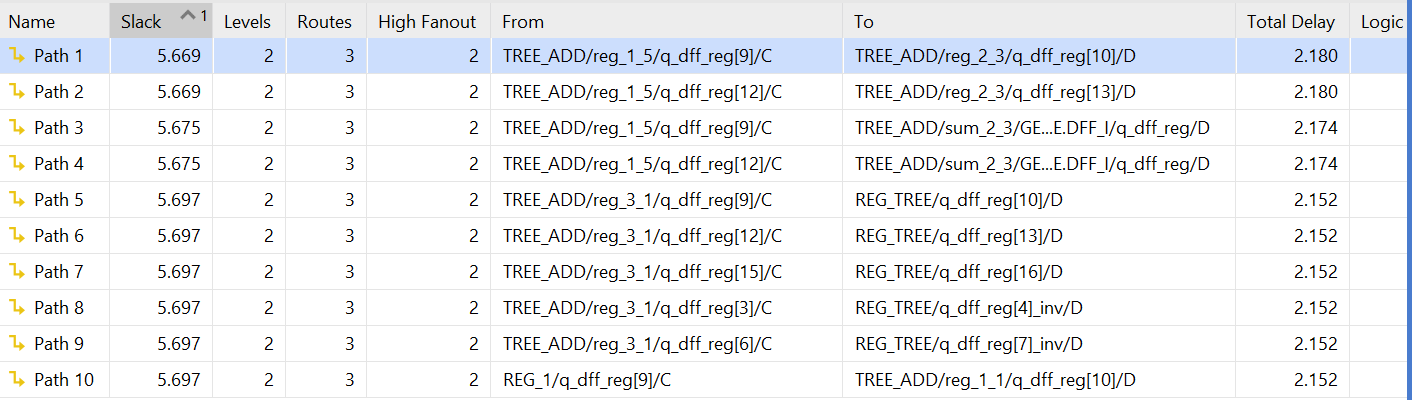
\includegraphics[width=\textwidth]{img/vivado/critical_path.png}
	\caption{Critical Path Report}
\end{figure}
We can state that the \textbf{Tree Adder} module has the most impact on the \textbf{critical path} so the addition of some registers in between the ripple carry adders and even the addition of the pipelines registers in the latter, during the project phase, were all \textbf{good project choices}.
\subsection{Resource Utilization Report}
The resource utilized by the architecture synthesized are the following:
\begin{figure}[H]
	\centering
	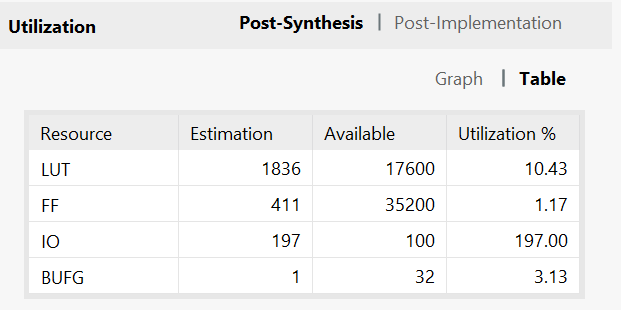
\includegraphics[width=0.6\textwidth]{img/vivado/utilization.png}
	\caption{Critical Path Report}
\end{figure}
As we can see the IO resource utilization is greater than the 100$\%$ of the available one (179 input pins and 16 output pins necessary). So it was not possible to head with the implementation phase with the Zybo Zynq 7000. We can also see that the LUT resource has been utilized by the roughly 10$\%$, so, with this numbers, the LUT optimization done has halved the LUT utilization and it was a \textbf{good project choice}.
\subsection{Power Consumption Report}
The power consumption report is the following:
\begin{figure}[H]
	\centering
	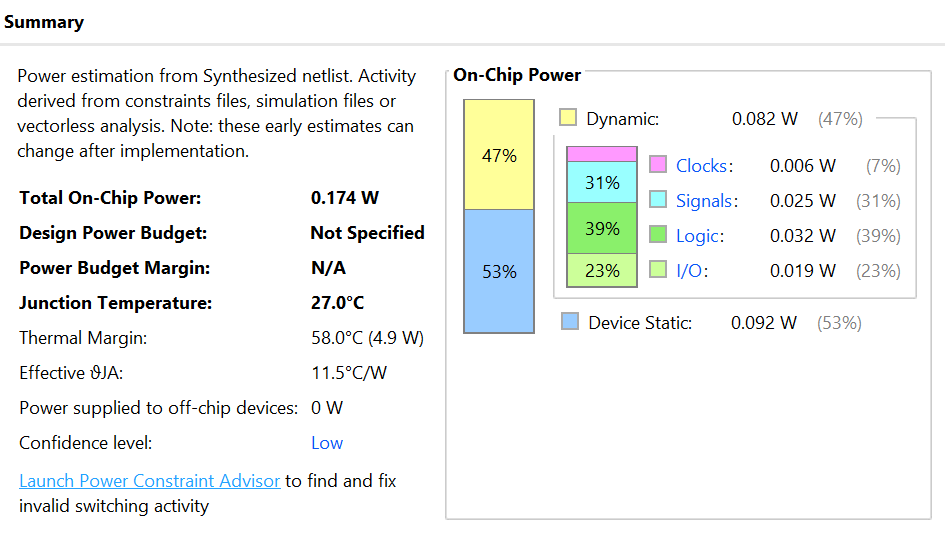
\includegraphics[width=0.8\textwidth]{img/vivado/power.png}
	\caption{Power Consumption Report}
\end{figure}
As we can see, a total of 0.174 W of Power are needed (with the standard settings suggested by Xilinx VIVADO), which is roughly divided equally between dynamic and static power. For the \textbf{Dynamic Power Consumption} the most relevant contributes are from the logic and signals.
\subsection{Warning Messages}
After the synthesis phase the following warning messages were shown:
\begin{figure}[H]
	\centering
	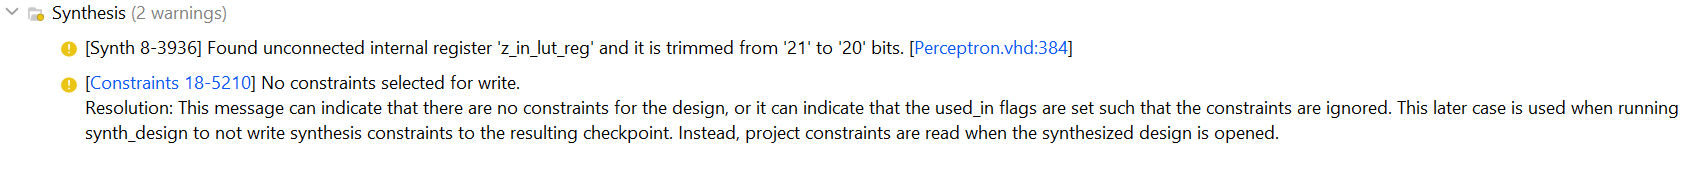
\includegraphics[width=\textwidth]{img/vivado/warnings.png}
	\caption{Warning Messages}
\end{figure}
So, let's analyse them:
\begin{itemize}
	\item \textbf{[Constraints 18-5210] No constraints selected for write}: this warning message was shown even during the laboratory classes and it can be ignored. 
	\item \textbf{[Synth 8-3936] Found unconnected internal register 'z$\_$in$\_$lut$\_$reg' and it is trimmed from '21' to '20' bits:} this warning message is due to the fact that to get the proper address on the lut, after the lut optimization, the first bit (the 21th) is the sign one and is used to perform just some additional operation, it has no relevance on the addressing of the lut.
\end{itemize}